\typeout{(body.tex)}

\begin{frame}
    \titlepage
\end{frame}

\section{memory layout}
\tikzset{
    program memory label/.style={font=\ttfamily},
    program memory box/.style={draw,rectangle,minimum width=5cm,fill=white},
    program memory highlight/.style={draw,rectangle,line width=1mm, draw=blue!80!black,opacity=.3,
        inner sep=0.5mm},
}

\newcommand{\programMemoryImage}{
\node[program memory box,minimum height=1cm,pattern=north west lines,pattern color=black!5!white] (kernel) {Used by OS};
\node[right=1mm of kernel.north east,program memory label] {0xFFFF FFFF FFFF FFFF};
\node[right=1mm of kernel.south east,program memory label] {0xFFFF 8000 0000 0000};
\node[program memory box, minimum height=.5cm, below=1cm of kernel] (stack) {Stack};
\node[right=1mm of stack.north east,program memory label] {0x7F\ldots{}};
\node[program memory box, minimum height=.5cm, below=1cm of stack] (heap) {Heap / other dynamic};
\node[program memory box, minimum height=.5cm, below=0mm of heap] (data) {Writable data};
\node[program memory box, minimum height=.5cm, below=0mm of data] (sdata) {Code + Constants};
\node[right=1mm of sdata.south east,program memory label] {0x0000 0000 0040 0000};
\coordinate (memBottom) at ($(sdata.south east) + (0mm, -2mm)$);
\begin{pgfonlayer}{bg}
\draw[pattern=north west lines, pattern color=black!40!white] (kernel.north west) rectangle (memBottom);
\end{pgfonlayer}
}
\newcommand{\programMemoryHighlight}[1]{
    \node[#1,program memory highlight] {};
}

\begin{frame}{a possible memory layout on Linux}
\begin{tikzpicture}
\programMemoryImage
    \begin{visibleenv}<2>
        \programMemoryHighlight{fit=(heap)}
        \node[right=1cm of heap,align=left] {grows upward \\ $\rightarrow$ new, malloc};
    \end{visibleenv}
    \begin{visibleenv}<3>
        \programMemoryHighlight{fit=(stack)}
        \node[right=1cm of stack,align=left] {$\rightarrow$ local variables allocated here \\ grows downward};
    \end{visibleenv}
\end{tikzpicture}
\end{frame}


\begin{frame}{stack v heap}
\begin{tabular}{ll}
stack & heap \\ \hline
compiler managed & programmer managed \\
values go out of scope & explicit free \\
within procedure only & outlives procedures \\
x86: grows down & x86: grows up \\
\end{tabular}
\end{frame}


\subsection{aside: address translation}
\begin{frame}{address translation}
\begin{tikzpicture}
\tikzset{
    every node/.style={font=\small},
}
\node[align=center,alt=<2>{draw=red,very thick,fill=red!10}{}] (progAAddr) {Program A \\ addresses \\ \myemph<3>{``virtual''}};
\begin{visibleenv}<2>
\node[align=left,below=.5cm of progAAddr] {\myemph{every address accessed} \\ instructions \textit{and} data};
\end{visibleenv}
%\node[below=1cm of progAAddr,align=center] (progBAddr) {Program B \\ addresses};
\node[draw, right=3cm of progAAddr,align=center,alt=<4>{draw=red,very thick,fill=red!10}] (translationA) { mapping \\ (set by OS) };
\begin{visibleenv}<4>
\node[align=left,below=.5cm of translationA] {stored in processor? \\ format?};
\end{visibleenv}
%\node[draw, right=3cm of progBAddr,align=center] (translationB) { mapping \\ (set by OS) };
\node[draw,rectangle split, rectangle split parts=6, anchor=north west,label={[align=center]north:real memory\\\myemph<3>{``physical''}}] (mem) at ([xshift=3cm]translationA.north east) {
    \nodepart{one}
    Program A code 
    \nodepart{two}
    Program B code
    \nodepart{three}
    Program A data
    \nodepart{four}
    Program B data
    \nodepart{five}
    OS data
    \nodepart{six}
    \ldots
};
\draw[-Latex,green,thick] (progAAddr) -- (translationA) (translationA.east) -- (mem.one west);
\draw[-Latex,green,thick] (translationA.east) -- (mem.three west);
%\draw[-Latex,blue,thick] (progBAddr) -- (translationB) (translationB.east) -- (mem.two west);
%\draw[-Latex,blue,thick] (translationB.east) -- (mem.four west);
%\node[thick,red,draw,anchor=north west] (error) at ([yshift=-.5cm]mem.south west) {trigger error};
%\draw[-Latex,green,thick] (translationA.east) -- (error.west);
%\draw[-Latex,blue,thick] (translationB.east) -- (error.west);
%\draw[-Latex,green,ultra thick,dotted] (translationA.east) -- (mem.five west);
%\draw[-Latex,blue,ultra thick,dotted] (translationB.east) -- (mem.five west);
\begin{visibleenv}<3>
\node[draw,thick,align=center,below=3cm of translationA] {
    program addresses are `virtual' \\
    real addresses are `physical'
};
\end{visibleenv}
\end{tikzpicture}
\end{frame}


\section{alloca}

\begin{frame}{alloca}
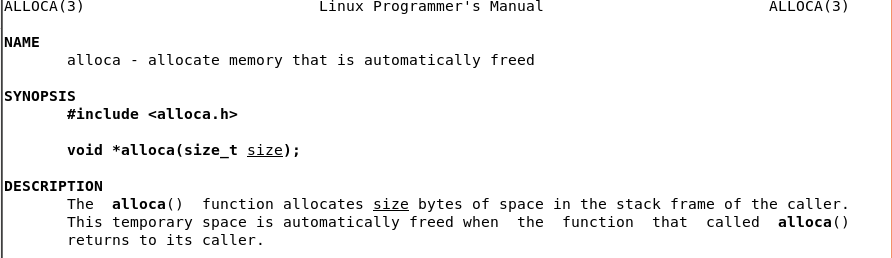
\includegraphics[width=\textwidth]{alloca-man}
\end{frame}

\begin{frame}{writing alloca}
\begin{itemize}
\item how is it possible to write this function???
\item allocating space without overwriting return address???
\end{itemize}
\end{frame}

\begin{frame}[fragile,label=histBSDAlloca]{an historical implementation}
\lstset{
    language=myasm,
    style=smaller,
    moredelim={**[is][\btHL<all:2>]{@2}{2@}},
    moredelim={**[is][\btHL<all:3>]{@3}{3@}},
    moredelim={**[is][\btHL<all:4>]{@4}{4@}},
}
\begin{itemize}
\item 386BSD (1990) 32-bit x86 implementation
\begin{itemize}\item converted to Intel syntax, some comments added\end{itemize}
\end{itemize}
\begin{lstlisting}
alloca:
    pop edx		/*  pop return addr */
    pop @2eax2@		/*  pop amount to allocate */
    mov	ecx, esp
    add	eax, 3		/*  round up to next word */
    and eax, 0xfffffffc
    sub @3esp3@,eax         /* adjust stack pointer for allocation */
    mov	eax,esp 	/* set ret. val. to base of
                               newly allocated space */
    push @4[ecx+8]4@	/* copy possible saved registers */
    push [ecx+4]
    push [ecx+0]
    push @2eax2@		/* dummy to pop at callsite */
    jmp	edx		/* "return" */
\end{lstlisting}
\begin{tikzpicture}[overlay,remember picture]
    \coordinate (placeLow) at ([yshift=2cm]current page.south);
    \coordinate (placeHigh) at ([yshift=5cm]current page.south);
    \tikzset{box/.style={draw=red,very thick,fill=white,anchor=south,align=left}}
    \begin{visibleenv}<2>
        \node[box] at (placeLow) {
            32-bit x86 calling convention: all args on stack
        };
    \end{visibleenv}
    \begin{visibleenv}<3>
        \node[box] at (placeHigh) {
            changing stack pointer \\
            how does caller access local variables on the stack? \\
            assumption: uses a base pointer instead\ldots
        };
    \end{visibleenv}
    \begin{visibleenv}<4>
        \node[box] at (placeHigh) {
            how do we know caller only saves 3 registers? \\
            we don't\ldots
        };
    \end{visibleenv}
\end{tikzpicture}
\end{frame}

\begin{frame}[fragile,label=modernAlloca]{a modern implementation: compiler built-in}
\lstset{
    language=C++,
    style=smaller,
    moredelim={**[is][\btHL<all:2>]{@2}{2@}},
    moredelim={**[is][\btHL<all:3>]{@3}{3@}},
    moredelim={**[is][\btHL<all:4>]{@4}{4@}},
}
\begin{lstlisting}
void foo(int N) {
    char *temp = alloca( N);
    bar(temp);
}
\end{lstlisting}
\lstset{
    language=myasm,
    style=smaller,
    moredelim={**[is][\btHL<all:2>]{@2}{2@}},
    moredelim={**[is][\btHL<all:3>]{@3}{3@}},
    moredelim={**[is][\btHL<all:4>]{@4}{4@}},
}
\begin{lstlisting}
foo: # @foo
  push @2rbp2@
  mov @2rbp, rsp2@
  movsxd rax, edi
  mov rdi, rsp
  add rax, 15
  and rax, -16
  sub rdi, rax
  mov rsp, rdi
  call bar
  mov @2rsp, rbp2@
  pop @2rbp2@
  ret
\end{lstlisting}
\end{frame}


\section{malloc and ::operator new}

\subsection{the interface}

\begin{frame}[fragile,label=mallocPrototype]{malloc}
\lstset{language=C++,style=small}
\begin{lstlisting}
void *malloc(size_t size);
\end{lstlisting}
\begin{itemize}
\item \texttt{void \*} --- generic pointer type
    \begin{itemize}
    \item in C --- converts implicitly to any pointer type
    \item in C++ --- requires cast
    \end{itemize}
\item \texttt{size\_t} --- integer type that holds size (in bytes)
\end{itemize}
\end{frame}

\begin{frame}[fragile,label=mallocUsage1]{typical malloc usage}
\lstset{language=C++,style=smaller}
\begin{lstlisting}
int *array;
...
array = malloc(number_of_elements * sizeof(*array))
// OR
array = malloc(number_of_elements * sizeof(int))
\end{lstlisting}
\hrule
\begin{lstlisting}
SomeType *item;
...
item = malloc(sizeof(*item));
// OR
item = malloc(sizeof(SomeType));
\end{lstlisting}
\hrule
note: in C++ (not C) would need casts
    \begin{itemize}
        \item \lstinline|array = (int*) malloc(...);|
    \end{itemize}
\end{frame}

\begin{frame}{malloc and free}
\begin{itemize}
\item free --- undo malloc's allocation
\end{itemize}
\end{frame}

\begin{frame}[fragile,label=newParts]{new}
\lstset{language=C++}
\begin{itemize}
    \item new does \myemph{two things} that can be done seperately
    \vspace{.5cm}
    \item allocate memory
        \begin{itemize}
        \item \texttt{operator new(sizeof(Foo))}
        \end{itemize}
    \item call constructors
        \begin{itemize}
        \item can do separately with ``placement new''
        \item \lstinline|new (somePtr) Foo(arguments);|
        \end{itemize}
    \end{itemize}
\end{frame}

\begin{frame}[fragile,label=placementNew]{``manually'' doing what new does}
\lstset{language=C++}
\begin{lstlisting}
Foo *foo = new Foo(1, 2, 3);
\end{lstlisting}
\hrule
\begin{lstlisting}
#include <memory>  // prototypes for operator new
...

// allocate space
Foo *foo = (Foo*) operator new(sizeof(Foo));

// call constructor
new (foo) Foo(1, 2, 3);
\end{lstlisting}
\end{frame}

\begin{frame}[fragile,label=placementNewVector]{implementing vector: create}
\lstset{language=C++,style=smaller}
\begin{lstlisting}
template <class T> class MyVector {
    ...
private:
    T * array;
    int size, capacity;
};

template <class T>
void MyVector::push_back(const T& other) {
    // increase array capacity if needed
    if (++size > capacity) { ... }

    // call copy constructor to create array[size-1]
    new (&array[size - 1]) T(other);
        // better than constructing all in advance and assigning
        // e.g. if vector of lists,
        //      don't allocate "extra" head/tail dummy nodes
}
\end{lstlisting}
\end{frame}

\begin{frame}[fragile,label=deleteParts]{delete}
\lstset{language=C++}
\begin{itemize}
    \item delete does \myemph{two things} that can be done seperately
    \vspace{.5cm}
    \item call destructors
        \begin{itemize}
        \item \lstinline|foo->~Foo();|
        \end{itemize}
    \item actually free memory
        \begin{itemize}
        \item \lstinline|operator delete(foo);|
        \end{itemize}
\end{itemize}
\end{frame}

\begin{frame}[fragile,label=manualDeleteVector]{implementing vector: destroy}
\lstset{language=C++,style=small}
\begin{lstlisting}
template <class T> class MyVector {
    ...
private:
    T * array;
    int size, capacity;
};

template <class T>
void MyVector::pop_back(const T& other) {
    size--;
    array[size].~T();
}
\end{lstlisting}
\end{frame}


\subsection{implementing malloc}

\begin{frame}{implementing malloc}
\begin{tabular}{ll}
malloc/new & OS allocation interfaces \\
16 byte or smaller allocations & minimum allocation/free: 4KB \\
100ish ns/allocation or free & microsecondish allocation/free \\
\end{tabular}
\begin{itemize}
\item OS manages memory in \textbf{4KB pages}
\item malloc/new ``batch'' small allocations into these big requests
\end{itemize}
\end{frame}

\begin{frame}{implementing malloc/free}
\begin{itemize}
    \item get \myemph{large allocations} from OS
    \item subdivide allocation --- need data structure to manage
    \begin{itemize}
        \item one idea: \myemph<2>{before what malloc/new returns}
        \item another idea: separate, e.g., hashtable on address
    \end{itemize} 
    \item lots of tricky choices:
    \begin{itemize}
        \item what if there are lots of non-contiguous free chunks?
        \item how to quickly find chunk of appropraite size
        \item \ldots
    \end{itemize}
\end{itemize}
\end{frame}

\tikzset{
    stackBox/.style={very thick},
    allocBox/.style={dashed,very thick,fill=blue!20},
    onStack/.style={thick,align=center},
    frameOne/.style={fill=blue!15},
    frameTwo/.style={fill=red!15},
    markLine/.style={blue!50!black},
    markLineB/.style={blue!90!black},
    hiLine/.style={red!90!black},
}

\begin{frame}[fragile,label=heapLayout]{one malloc/free impl.}
\begin{tikzpicture}
\node[anchor=north east] (code) at (-1,0) {
\begin{lstlisting}
struct AllocInfo {
  int size;
  // for alloc'd:
  AllocInfo *prev;
  AllocInfo *next;
};
\end{lstlisting}
};

\tikzset{
    isSize/.style={alt=<3>{fill=red!10}},
    isNextPrev/.style={alt=<2>{fill=red!10}},
}

\tikzset{xscale=0.9}
\begin{scope}[overlay,xshift=.5cm]
    \draw[stackBox,fill=black!20] (0, 1) rectangle (3, -7);

    \draw[onStack] (0, 1) rectangle (3, 0) node[midway,font=\small,align=center] {free space};
    \draw[onStack,fill=white,isNextPrev] (0, -0.0) rectangle (3, -0.5) node[midway,font=\small] (freeANext) {next};
    \draw[onStack,fill=white,isNextPrev] (0, -0.5) rectangle (3, -1.0) node[midway,font=\small] (freeAPrev) {prev};
    \draw[onStack,fill=white,isSize] (0, -1.0) rectangle (3, -1.5) node[midway,font=\small] (freeASize) {size};

    \draw[very thick, red, rounded corners] (0, 1) rectangle (3, -1.5);

    \draw[onStack,fill=blue!20] (0, -1.5) rectangle (3, -3.0) node[midway,font=\small,align=center] (freeBAlloc) {new'd object};
    \draw[onStack,fill=white,isSize] (0, -3.0) rectangle (3, -3.5) node[midway,font=\small] (freeBSize) {size};
    
    \draw[very thick, red, rounded corners] (0, -1.5) rectangle (3, -3.5);

    \draw[onStack] (0, -3.5) rectangle (3, -5.0) node[midway,font=\small] {free space};
    \draw[onStack,fill=white,isNextPrev] (0, -5.0) rectangle (3, -5.5) node[midway,font=\small] (freeCNext) {next};
    \draw[onStack,fill=white,isNextPrev] (0, -5.5) rectangle (3, -6.0) node[midway,font=\small] (freeCPrev) {prev};
    \draw[onStack,fill=white,isSize] (0, -6.0) rectangle (3, -6.5) node[midway,font=\small] (freeCSize) {size};
    
    \draw[very thick, red, rounded corners] (0, -3.5) rectangle (3, -6.5);
    
    \draw[-Latex,blue,thick] (freeAPrev) -- ++(1.75cm,0cm) |- (freeCSize);
    \draw[-Latex,blue,thick] (freeCNext) -- ++(2.00cm,0cm) |- (freeASize);
    \draw[-Latex,blue,thick,opacity=0.5] (freeCPrev) -- ++(1.25cm,0cm) -- ++(0cm,-2cm);
    \draw[-Latex,blue,thick,opacity=0.5] (freeANext) -- ++(1.75cm,0cm) -- ++(0cm,2cm);
\end{scope}
\begin{visibleenv}<2>
    \node[below=.5cm of code,align=left] {
        keep \myemph{linked list} of \\ available chunks of memory
    };
\end{visibleenv}
\begin{visibleenv}<3>
    \node[below=.5cm of code,align=left] {
        keep \myemph{sizes} before allocations \\
        maybe need less with \texttt{delete}?
    };
\end{visibleenv}
\begin{visibleenv}<4>
    \node[below=.5cm of code,align=left] {
        merge adjacent free allocations \\
        (if any)
    };
    \draw[-Latex,line width=3pt,black!50] (4.5,-2.25) -- (5.5,-2.25) node[black,midway,above,font=\small\tt] {free};
    \begin{scope}[overlay,xshift=6cm,name prefix=sec-]
        \draw[stackBox,fill=black!20] (0, 1) rectangle (3, -7);

        \draw[onStack] (0, 1) rectangle (3, -5.0) node[midway,font=\small] {free space};
        \draw[onStack,fill=white] (0, -5.0) rectangle (3, -5.5) node[midway,font=\small] (freeCNext) {next};
        \draw[onStack,fill=white] (0, -5.5) rectangle (3, -6.0) node[midway,font=\small] (freeCPrev) {prev};
        \draw[onStack,fill=white] (0, -6.0) rectangle (3, -6.5) node[midway,font=\small] (freeCSize) {size/free};
        
        \draw[-Latex,blue,thick,opacity=0.5] (freeCPrev) -- ++(1.25cm,0cm) -- ++(0cm,-2cm);
        \draw[-Latex,blue,thick,opacity=0.5] (freeCNext) -- ++(1.75cm,0cm) -- ++(0cm,2cm);
    \end{scope}
\end{visibleenv}
\end{tikzpicture}
\end{frame}

\begin{frame}{tough malloc/free choices}
    \begin{itemize}
    \item quickly finding free blocks of right size
    \item avoiding large amounts of small, free spaces
        \begin{itemize}
        \item enough free memory, but not usable?
        \item ``fragmentation''
        \end{itemize}
    \item extra overhead (sizes, next/prev pointers, \ldots)
    \vspace{.5cm}
    \item how many lists of free blocks?
    \item different lists for different sizes?
    \item return first block or best sizes block? in between?
    \end{itemize}
\end{frame}


\section{realloc}

\begin{frame}[fragile,label=realloc]{realloc}
\lstset{language=C++,style=small}
\begin{itemize}
    \item \lstinline|void *realloc(void *pointer, size_t size)|
    \item either:
        \begin{itemize}
        \item \myemph<2>{changes the size} of the allocation at \lstinline|pointer|, or
        \item \myemph<3>{allocates new space}, \myemph<3>{copies data} from \lstinline|pointer| there, \myemph<4>{free} (old) pointer
        \end{itemize}
    \item returns the new space (if any, or \lstinline|pointer| otherwise)
\end{itemize}
\begin{tikzpicture}
\tikzset{
    stackBox/.style={very thick},
    allocBox/.style={dashed,very thick,fill=blue!20},
    onStack/.style={thick,align=center},
    frameOne/.style={fill=red!25},
    frameTwo/.style={fill=blue!10},
    frameThree/.style={pattern color=blue,pattern=crosshatch},
    markLine/.style={blue!50!black},
    markLineB/.style={blue!90!black},
    hiLine/.style={red!90!black},
    >=Latex,
}
    \draw[stackBox] (0, 0) rectangle (2, -4);
    \draw[onStack,frameOne] (0, -.5) rectangle (2, -1);
    \draw[onStack,frameTwo] (0, -3) rectangle (2, -4);
    \draw[onStack,frameTwo] (0, -1.5) rectangle (2, -2.75);

    \begin{visibleenv}<2>
        \draw[red,thick,rounded corners] (-.25,.25) rectangle (5.25,-4.25);
    \end{visibleenv}
    \begin{visibleenv}<3>
        \begin{scope}[xshift=7cm]
        \draw[red,thick,rounded corners] (-.25,.25) rectangle (5.25,-4.25);
        \end{scope}
    \end{visibleenv}
    \begin{visibleenv}<4>
        \begin{scope}[xshift=7cm]
        \draw[red,thick,rounded corners] (2.75,.25) rectangle (8.25,-4.25);
        \end{scope}
    \end{visibleenv}

    \foreach \x in {2.5,9.5,12.5} {
        \draw[->,ultra thick,black!50] ($(\x, -2) + (-.25,0)$) -- ++(.5cm,0cm);
    }

    \draw[stackBox] (3, 0) rectangle (5, -4);
    \draw[onStack,frameOne] (3, -.5) rectangle (5, -1.25);
    \draw[onStack,frameTwo] (3, -3) rectangle (5, -4);
    \draw[onStack,frameTwo] (3, -1.5) rectangle (5, -2.75);

    \begin{scope}[xshift=7cm]
    \draw[stackBox] (0, 0) rectangle (2, -4);
    \draw[onStack,frameOne] (0, -.5) rectangle (2, -1);
    \draw[onStack,frameTwo] (0, -1.1) rectangle (2, -1.9);

    \draw[stackBox] (3, 0) rectangle (5, -4);
    \draw[onStack,frameOne,dotted] (3, -.5) rectangle (5, -1);
    \draw[onStack,frameTwo] (3, -1.1) rectangle (5, -1.9);
    \draw[onStack,frameOne] (3, -2) rectangle (5, -3.25);
    \draw[onStack,dotted] (3, -2) rectangle (5, -2.5);

    \draw[stackBox] (6, 0) rectangle (8, -4);
    \draw[onStack,frameTwo] (6, -1.1) rectangle (8, -1.9);
    \draw[onStack,frameOne] (6, -2) rectangle (8, -3.25);
    \end{scope}
\end{tikzpicture}
\end{frame}

\begin{frame}{some realloc gotchas}
    \begin{itemize}
    \item need to \myemph{use return value} --- data might have moved!
    \item need to worry about \myemph{other copies of the pointer}
    \end{itemize}
\end{frame}

\begin{frame}{realloc runtime}
    \begin{itemize}
    \item copy: $\Theta(n)$
    \item in place: $\Theta(1)$
    \end{itemize}
\end{frame}


\section{memory hierarchy}

\subsection{overview picture and performance}

\begin{frame}{2004 CPU}
    \begin{tikzpicture}[scale=1.25]
\clip (1,0) rectangle (14, 7);
\node[anchor=south west] (diePhoto) at (0,0) {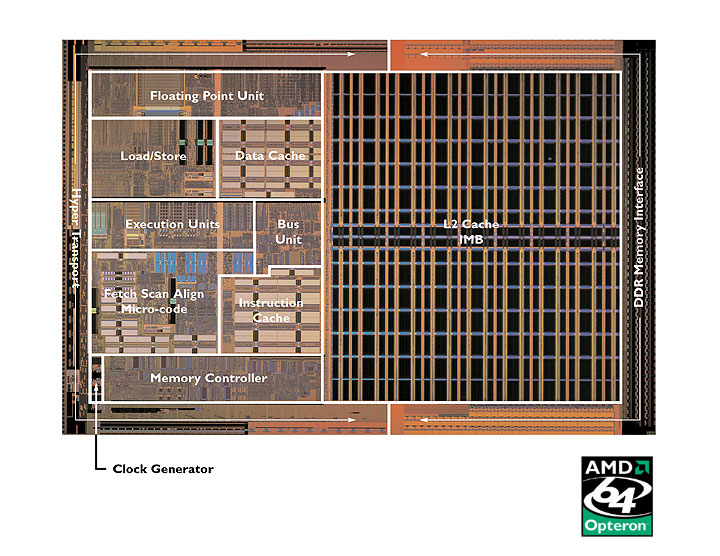
\includegraphics[width=11.25cm]{Opteron_die_labelled.jpg}};
%\draw[red] (0, 0) grid (9,7);
    \newcommand{\pyrShift}{0.5cm}
\onslide<2->{
    \draw[fill=red,opacity=0.6] (1.9,6.2) rectangle (2.4,5.8);
    \draw[fill=red,opacity=0.6] (1.7,4.2) rectangle (1.9,4.6);

    \begin{scope}[xshift=\pyrShift]
    \draw[fill=red!60!white] (10,7) -- (9.75,6.5) -- (10.25,6.5) -- cycle;
    \node[anchor=west] at (10.1, 6.75) {Registers};
    \end{scope}
}
\onslide<3->{
    %\draw[fill=orange,opacity=0.6] (2.95,2.7) rectangle (4.2,3.6);
    \draw[fill=orange,opacity=0.6] (2.95,2.7) -| (4.2,3.8) -| (3.6,3.65) -- (2.95,3.65) -- (2.95,2.7);
    \draw[fill=orange,opacity=0.6] (2.95,4.6) rectangle (4.2,5.6);

    \begin{scope}[xshift=\pyrShift]
    \draw[fill=orange!60!white] (9.5,6) -- (9.75,6.5) -- (10.25,6.5) -- (10.5,6) -- cycle;
    \node[anchor=west] at (10.35,6.25) {L1 cache};
    \end{scope}
}
\onslide<4->{
    \draw[fill=yellow,opacity=0.6] (4.2,2.1) rectangle (7.9,6.25);
    
    \begin{scope}[xshift=\pyrShift]
    \draw[fill=yellow!60!white] (9.25,5.5) -- (9.5,6) -- (10.5,6) -- (10.75,5.5) -- cycle;
    \node[anchor=west] at (10.6,5.75) {L2 cache};
    \end{scope}
}
\onslide<6->{
    \begin{scope}[xshift=\pyrShift]
    \draw[pattern color=green!60!white,pattern=north west lines] (9.0,5.) -- (9.25,5.5) -- (10.75,5.5) -- (11.,5.) -- cycle;
    \node[anchor=west] at (10.85,5.25) {L3 cache};
    \draw[fill=blue!60!white] (8.5,4.) -- (9.,5.) -- (11,5.) -- (11.5,4.) -- cycle;
    \node[anchor=center,align=center] at (10.,4.5) {main\\memory};
    \end{scope}
}
\onslide<7->{
    \begin{scope}[xshift=\pyrShift]
    \fill[white,opacity=0.9] (7.0,4.5) rectangle (8.4,10.0);
    \begin{scope}[font=\fontsize{10}{11}\selectfont]
        \node[anchor=east] at (9.,6.75) {$<1$ ns};
        \node[anchor=east] at (9.,6.25) {$\sim1$ ns};
        \node[anchor=east] at (9.,5.75) {$\sim5$ ns};
        \node[anchor=east] at (9.,5.25) {$\sim20$ ns};
        \node[anchor=east] at (9.,4.75) {$\sim100$ ns};
    \end{scope}
    \end{scope}
}
\end{tikzpicture}
    \imagecredit{Image: approx 2004 AMD press image of Opteron die; \\ approx register location via chip-architect.org (Hans de Vries)}
\end{frame}

% FIXME: colors consistent with previous slide
\begin{frame}{memory hierarchy overview}
\begin{tikzpicture}
    \begin{scope}[xscale=0.8,yscale=1.2]
        \draw[ultra thick] (-1,-1) -- (-7, -7) -- (7, -7) -- (1,-1) -- cycle;
        \foreach \x/\lbl in {
                2/registers,
                3/{level 1 (L1) cache},
                4/{level 2 (L2) cache},
                5/{level 3 (L3) cache},
                6/main memory,
                7/hard disk or SSD
            } {
            \draw[thick] (-\x, -\x) -- (\x, -\x);
            \node[anchor=south] at (0, -\x) {\lbl};
        }
        \tikzset{
            >=Latex
        }
        \draw[->,thick] (3, -2) -- (6, -5) node[below right] {bigger and slower};
        \node[anchor=west] at (3, -2) {faster and smaller};
    \end{scope}
\end{tikzpicture}
\end{frame}

\begin{frame}{memory hierarchy goal}
    \begin{itemize}
    \item size of largest, slowest storage
    \item speed of smallest, fastest storage
        \vspace{.5cm}
    \item not actually possible, but can get pretty close due to locality
    \end{itemize}
\end{frame}

\begin{frame}{memory hierarchy numbers}
from a system like my desktop: \\
    {\small (note: multiple parallel accesses and/or sequential accesses needed to achieve maximum bandwidths)} \\
\begin{tabular}{l|lll}
level & time/access & maximum read bandwidth \\ \hline
registers & 0.3 ns & $\sim$ 645 GB/s (per core)\\
L1 cache & 1.2 ns & $\sim$ 199 GB/s (per core) \\
L2 cache & 3.6 ns & $\sim$ 110 GB/s (per core)\\
L3 cache & $\sim$ 13 ns & $\sim$ 54 GB/s \\
main memory & $\sim$ 64 ns & $\sim$ 25 GB/s \\
hard disk & $\sim$ 5$\;$000$\;$000 ns & $\sim$ 0.1 GB/s \\
\end{tabular}
\end{frame}



\subsection{caches}

\begin{frame}{caches}
    \begin{itemize}
    \item caches --- fast memory that holds\\
        \myemph{recently accessed values from main memory} and \\
        \myemph{values near recently accessed values from main memory}
    \item idea: program thinks it accesses main memory\ldots \\
        but most accesses take `shortcut' to cache
    \end{itemize} 
\end{frame}

\begin{frame}[fragile,label=observeCaches]{observing caches}
\lstset{
    language=C++,style=smaller
}
\begin{lstlisting}
unsigned run(int count) {
    unsigned index = 0;
    for (unsigned j = 0; j < count; ++j) {
        index = array[index];
    }
    return index;
}

// setup to access array with no easily observed pattern
    // NB: 103 will be relatively prime, so this accesses
    //     every element of the array
void setup(int size) {
    for (unsigned i = 0; i < size; ++i) {
        array[i] = ((i + 1) * 103) % size;

    }
}
\end{lstlisting}
\end{frame}

\begin{frame}{observing caches}
    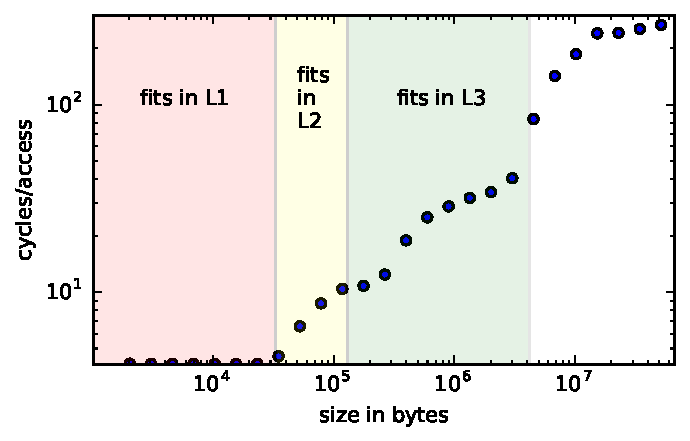
\includegraphics[width=\textwidth]{size-v-cycles}
\end{frame} 


\section{locality}

\subsection{types of locality}

\begin{frame}[label=localityIntro]{memory hierarchy assumptions}
\begin{itemize}
    \item \myemph{temporal locality} \\
        ``if a value is accessed now, it will be accessed again soon''
        \begin{itemize}
        \item caches should keep \myemph{recently accessed values}
        \end{itemize}
    \vspace{.5cm}
    \item \myemph{spatial locality} \\
        ``if a value is accessed now, adjacent values will be accessed soon''
        \begin{itemize}
        \item caches should \myemph{store adjacent values at the same time}
        \end{itemize}

    \vspace{1cm}
    \item natural properties of programs --- think about loops
\end{itemize}
\end{frame}

\begin{frame}[fragile,label=localityExamples]{locality examples}
\lstset{language=C,style=small}
\begin{lstlisting}
double computeMean(int length, double *values) {
    double total = 0.0;
    for (int i = 0; i < length; ++i) {
        total += values[i];
    }
    return total / length;
}
\end{lstlisting}
\begin{itemize}
    \item temporal locality: machine code of the loop
    \item spatial locality: machine code of most consecutive instructions
    \item temporal locality: {\tt total}, {\tt i}, {\tt length} accessed repeatedly
    \item spatial locality: {\tt values[i+1]} accessed after {\tt values[i]}
\end{itemize}
\end{frame}


\subsection{locality and performance}

\begin{frame}[fragile,label=loopOrderEx]{locality example}
\lstset{language=C++,style=smaller}
\begin{tikzpicture}
\node (goodCode){
\begin{lstlisting}
for(int i = 0; i < 1024; i++)
  for(int j = 0; j < 1024; j++)
    array[i][j] = 0;
for(int c = 0; c < 1024; c++)
  for(int i = 0; i < 1024; i++)
    for(int j = 0; j < 1024; j++)
      array[i][j]++;
for(int i = 0; i < 1024; i++)
  for(int j = 0; j < 1024; j++)
    sum += array[i][j];
\end{lstlisting}
};
\node[below=0cm of goodCode] {on my laptop: 0.31 s};
    \draw (goodCode.north east) -- (goodCode.south east);
\node[right=0cm of goodCode] (badCode) {
\begin{lstlisting}
for(int j = 0; j < 1024; j++)
  for(int i = 0; i < 1024; i++)
    array[i][j] = 0;
for(int c = 0; c < 1024; c++)
  for(int j = 0; j < 1024; j++)
    for(int i = 0; i < 1024; i++)
       array[i][j]++;
for(int j = 0; j < 1024; j++)
  for(int i = 0; i < 1024; i++)
    sum += array[i][j];
\end{lstlisting}
};
    \node[below=0cm of badCode] {on my laptop: 2.30 s};
\end{tikzpicture}
\end{frame}


\subsection{locality and data structures}

\begin{frame}{data structure locality}
\begin{tikzpicture}
    \tikzset{
        >=Latex,
        list node/.style={
            on chain,draw,rectangle split, rectangle split parts=2,
            rectangle split horizontal, join
        }
    }
    \matrix[tight matrix,nodes={minimum height=.5cm}] (the array) {
        1 \& 2 \& 3 \& |[draw=none]| \ldots \& 10 \\
    };
    \matrix[tight matrix,
        column 1/.style={nodes={draw=none,font=\tt\small,text width=2cm}},
        column 2/.style={nodes={draw,font=\tt\small,text width=2cm}},
        anchor=west,
        ] (the array layout) at ([xshift=5cm]the array.east) {
        0x1000 \& 1 \\
        0x1008 \& 2 \\
        0x1010 \& 3 \\
        0x1018 \& 4 \\
        \ldots \& |[draw=none]| \ldots \\
    };

    \begin{scope}[start chain=going right,
            every join/.style={->,thick},
        ]
        \node[list node,anchor=north west] at ([yshift=-2cm]the array.south west) { 1 };
        \node[list node] { 2 };
        \node[list node] { 3 };
        \node[on chain,join] { \ldots };
        \node[list node] { 10 };
    \end{scope}

    \matrix[tight matrix,
        column 1/.style={nodes={draw=none,font=\tt\small,text width=2cm}},
        column 2/.style={nodes={draw,font=\tt\small,text width=2cm}},
        anchor=north west,
        ] (list layout) at ([yshift=-1cm]the array layout.south west) {
        0x1000 \& 1 \\
        0x1008 \& 0x1050 \\
        \ldots \& |[draw=none]| \ldots \\
        0x1020 \& 3 \\
        0x1028 \& 0x1060 \\
        \ldots \& |[draw=none]| \ldots \\
        0x1050 \& 2 \\
        0x1058 \& 0x1020 \\
        0x1060 \& 4 \\
        \ldots \& |[draw=none]| \ldots \\
    };
\end{tikzpicture}
\end{frame}


\section{performance trends}

% FIXME:

\section{C strings and C string functions}

\subsection{C string representation}


\begin{frame}[fragile,label=cStrings]{strings in C}
\lstset{language=C++,style=smaller}
\begin{tikzpicture}
    \tikzset{
        mybox part/.style={minimum width=2cm,font=\scriptsize,align=left,fill=black!10!white},
        mybox/.style={draw,rectangle,mybox part},
        mycodebox/.style={draw,rectangle,mybox part,fill=white},
        mylabel/.style 2 args={label={[label distance=-1mm,inner sep=1mm,fill=white,draw,rectangle,font=\footnotesize,visible on=#2]90:#1}},
        myline/.style={line width=1pt,-latex},
    }
    \node[mycodebox] (code) {
\begin{lstlisting}[style=smaller]
int main() {
   const char *hello = "Hello World!";
   ...
}
\end{lstlisting}
    };
    \node[left=2cm of code,mylabel={\texttt{hello} (on stack/register)}{<1->},mybox] (ptr) {0x4005C0};
    \matrix[matrix of nodes,
        mylabel={read-only data}{<1->},below=1.5cm of ptr,mybox,
        nodes={draw,rectangle,minimum width=0mm,minimum height=.5cm, inner sep=0mm,anchor=south,
               font=\tt\scriptsize\addfontfeatures{Mapping=}},
        xshift=3cm,
        inner sep=0mm,outer sep=0mm,
    ] (data) {
        \sf\ldots\&'H'\&'e'\&'l'\&'l'\&'o'\&'\verb*| |'\&
        'W'\&'o'\&'r'\&'l'\&'d'\&'!'\&'\textbackslash0'\&\sf\ldots\\
    };

    \draw[-latex,very thick] (ptr) -- (data-1-2);

    \begin{visibleenv}<2>
    \matrix[below=.5cm of data,xshift=3cm,tight matrix,
        column 1/.style={nodes={draw=none,text width=3cm,font=\tt\fontsize{8}{9}\selectfont}},
        column 2/.style={nodes={text width=2cm,font=\tt\fontsize{8}{9}\selectfont}},
        column 3/.style={nodes={draw=none,blue,text width=1.5cm,font=\tt\fontsize{8}{9}\selectfont}},
        row 1/.style={nodes={font=\normalfont\bfseries\fontsize{8}{9}\selectfont,draw=none}},
    ] (memory) {
        address(es) \& value \\
        0x4005c0 \& 0x48 \& 'H' \\
        0x4005c1 \& 0x65 \& 'e' \\
        0x4005c2 \& 0x6c \& 'l' \\
        0x4005c3 \& 0x6c \& 'l' \\
        0x4005c4 \& 0x6f \& 'o' \\
        \ldots \& |[draw=none]| \ldots \\
        0x4005ca \& 0x21 \& '!' \\
        0x4005cb \& 0x00 \& '\textbackslash0' \\
        \ldots \& \ldots \\
        0x7fff3488-8f \& 0x4005c0 \& hello \\
    };
    \draw[thick,decorate,decoration={brace,mirror}] (memory-2-1.north west) -- (memory-9-1.south west) node[left,midway,font=\small] {string (constant data)};
    \draw[thick,decorate,decoration={brace,mirror}] (memory-10-1.north west) -- (memory-11-1.south west) node[left,midway,font=\small] {pointer (on stack)};

    \end{visibleenv}

\end{tikzpicture}
\end{frame}



% FIXME: strings allocated on stack

\subsection{strlen, strcpy, strcat}

\begin{frame}[fragile,label=cStrLib]{C standard library functions}
\lstset{
    language=C++,style=small
}
\begin{itemize}
    \item header file: \texttt{string.h}
    \vspace{.5cm}
    \item \lstinline|size_t strlen(const char* s)| --- number of chars in s
    \item \lstinline|char *strcpy(char *s1, const char *s2)| --- copy \texttt{s2} to \texttt{s1}, return \texttt{s1}
    \item \lstinline|char *strcat(char *s1, const char *s2)| --- append \texttt{s2} to \texttt{s1}, return \texttt{s1}
\end{itemize}
\end{frame}

\begin{frame}[fragile,label=strlenImpl]{implementing strlen}
\lstset{
    language=C++,style=small
}
\begin{lstlisting}
size_t strlen(const char* s) {
    size_t i = 0;
    while (s[i] != '\0')
        i += 1;
    return i;
}
\end{lstlisting}
\end{frame}

\begin{frame}[fragile,label=strcpyReadOnly]{a strcpy inquiry (1)}
\lstset{
    language=C++,style=small
}
\begin{lstlisting}
char *hello = "Hello!";
char *bye = "Bye!";
strcpy(bye, hello);
\end{lstlisting}
\begin{visibleenv}<2->
\hrule
C result: \myemph{Segmentation fault}
C++ result: compile error, \texttt{"Hello!"} is const
\end{visibleenv}
\end{frame}

\begin{frame}[fragile,label=strcpyTooSmall]{a strcpy inquiry (2)}
\lstset{
    language=C++,style=small
}
\begin{lstlisting}
const char *hello = "Hello!";
char bye[5] = {'B', 'y', 'e', '!', '\0'}; // or "Bye!" (same effect)
strcpy(bye, hello);
\end{lstlisting}
\hrule
\begin{visibleenv}<2->
same as:
\begin{lstlisting}
bye[0] = 'H'; bye[1] = 'e'; bye[2] = 'l'; bye[3] = 'l'; bye[4] = 'o';
bye[5] = '!'; bye[6] = '\0';
\end{lstlisting}
goes \myemph{out of bounds!}
\end{visibleenv}
\end{frame}

\begin{frame}[fragile,label=strcpyTooSmall]{a strcpy inquiry (3)}
\lstset{
    language=C++,style=small
}
\begin{lstlisting}
void foo() {
    const char *hello = "Hello!";
    char *dest = malloc(strlen(hello) + 1);
    strcpy(dest, hello);
    doSomethingWith(dest);
}
\end{lstlisting}
\hrule
\begin{visibleenv}<2->
\myemph{probably leaks memory}
\end{visibleenv}
\end{frame}


\subsection{code with memory leaks}

\begin{frame}[fragile,label=memLeakCode]{some code with memory leaks}
\lstset{language=C++,style=smaller}
\begin{lstlisting}
// allocate a space in memory for result
char *result = malloc (sizeof (*result));
int i = 1;
*result = '\0';
while (i < argc) {  // while there are still args
    char *s = malloc (sizeof (*s) *
            (strlen(result) + strlen(argv[i]) + 1));
    strcpy (s, result);
    strcat (s, argv[i]);
    result = s;
    i++;
}
printf ("Concatenation: %s\n", result);
\end{lstlisting}
\end{frame}


\begin{frame}[fragile,label=memLeakCodeFixed]{some code with memory leaks}
\lstset{language=C++,style=smaller,
    moredelim={**[is][\btHL<all:2>]{@2}{2@}},
    }
\begin{lstlisting}
// allocate a space in memory for result
char *result = malloc (sizeof (*result));
int i = 1;
*result = '\0';
while (i < argc) {  // while there are still args
    char *s = malloc (sizeof (*s) *
            (strlen(result) + strlen(argv[i]) + 1));
    strcpy (s, result);
    strcat (s, argv[i]);
    @2free(result);2@
    result = s;
    i++;
}
printf ("Concatenation: %s\n", result);
\end{lstlisting}
exercise: why \texttt{result} and not \texttt{s}?
\end{frame}


\begin{frame}{memory leak finding}
    \begin{itemize}
    \item idea: look at all pointers on stack, in global variables
    \begin{itemize}
        \item and all pointers contained in objects those reference
        \item and \ldots
    \end{itemize}
    \item and compare to list of all allocated objects
    \vspace{.5cm}
    \item done by tools like Valgrind Memcheck or AddressSanitizer
    \end{itemize}
\end{frame}


\section{where Big-Oh breaks}

\begin{frame}{recall: big-oh matters}
    \begin{itemize}
    \item not useful for fine-grained analysis
    \item assumption: operations take the same amount of time
        \begin{itemize}
        \item caches? --- not taken into account
        \item different versions of instructions
        \item \ldots
        \end{itemize}
    \end{itemize}
\end{frame}


\section{tail recursion and iterative methods}

\begin{frame}[fragile,label=recurseToTail]{recursion to tail recursion}
\lstset{language=C++,style=smaller}
\begin{lstlisting}
int factorial_recursive(int x) {
    if (x <= 1)
        return 1;
    else
        return x * factorial_recursive(x-1);
}
\end{lstlisting}
\hrule
\begin{lstlisting}
int factorial_tail_recursive(int x, int y = 1) {
    if (x <= 1)
        return y;
    else
        return factorial_tail_recursive(x-1, x*y);
}
\end{lstlisting}
\end{frame}

\begin{frame}[fragile,label=noCall]{tail recursion: avoiding call}
\lstset{language=myasm,style=smaller,
        moredelim={**[is][\btHL<all:2>]{@2}{2@}}}
}
\begin{lstlisting}
factorial_tail_recursive:
  cmp edi, 1
  jle .L4
.L2:
  imul esi, edi
  sub edi, 1
  @2jmp factorial_tail_recursive2@
  // same effect as:
  // call factorial_tail_recursive
  // ret
.L4:
  mov eax, esi
  ret
\end{lstlisting}
\end{frame}

\begin{frame}{tail recursion}
\begin{itemize}
    \item saves lots of stack space ($\Theta(x)$ space to $\Theta(1)$ space)
    \item easier for compilers to do
    \vspace{.5cm}
    \item ``tail'' requirement: must be last thing to do
    \item \ldots so it's okay to return directly to caller
\end{itemize}
\end{frame}

\begin{frame}[fragile,label=tailToLoop]{tail recursion to loop}
\lstset{language=C++,style=smaller}
\begin{lstlisting}
int factorial_tail_recursive(int x, int y = 1) {
    if (x <= 1)
        return y;
    else
        return factorial_tail_recursive(x-1, x*y);
}
\end{lstlisting}
\hrule
\begin{lstlisting}
int factorial_loop(int x) {
    int y = 1;
    while (x > 1) {
        y *= x;
        x--;
    }
    return y;
}
\end{lstlisting}
\end{frame}

